% Lecture Template for ME3001-001-Tristan Hill - Spring 2020
% Mechanical Engineering Analysis with MATLAB
% Ordinary Differential Equations - Topic 1

% I am finally converting my stuff to BEAMER

% Document settings



% !TEX TS-program = xelatex
% !TEX encoding = UTF-8 Unicode

% Lecture Template for ME3001-001-Tristan Hill - Spring 2017 - Fall 2017 - Fall 2020
% Mechanical Engineering Analysis with MATLAB
% Module 4 - ODE Applications 
% Topic 1 - Review and Classification  

\documentclass[fleqn]{beamer} % for presentation (has nav buttons at bottom)

\usepackage{/home/thill/Documents/lectures/analysis_lectures/analysis_lectures}

\newcommand{\MNUM}{5\hspace{2mm}} % Module number
\newcommand{\TNUM}{1\hspace{2mm}} % Topic number 
\newcommand{\moduletitle}{Systems of Linear Equations} % Titles and Stuff
\newcommand{\topictitle}{Linear Systems Review} 

\newcommand{\sectiontitleI}{What is a Differential Equation?} % More Titles and Stuff
\newcommand{\sectiontitleII}{Standard Form of an ODE}
\newcommand{\sectiontitleIII}{Classification}
\newcommand{\sectiontitleIV}{Example}


\author{ME3001 - Mechanical Engineering Analysis}
\title{Module \MNUM - \moduletitle}
\date{Mechanical Engineering\vspc Tennessee Technological University}

\begin{document}

\lstset{language=MATLAB,basicstyle=\ttfamily\small,showstringspaces=false}

\frame{\titlepage \center\begin{framed}\Large \textbf{Topic \TNUM - \topictitle}\end{framed} \vspace{5mm}}

% Section 0 - Outline
\frame{
	
	\large \textbf{Topic \TNUM - \topictitle} \vspace{3mm}\\
	
	\begin{itemize}
	
		\item \sectiontitleI    \vspc % Section I
		\item \sectiontitleII 	\vspc % Section II
		\item \sectiontitleIII 	\vspc %Section III
		\item \sectiontitleIV 	\vspc %Section IV
	
	\end{itemize}

}


\section{Definitions}

\subsection{What is a Differential Equation?}

\frame{

  \frametitle{What is a Differential Equation?}
  {\it Definition:\vspace{3mm}\\}
  A {\bf differential equation} is an equation which describes a function \vspace{3mm}\\and one or more of its \underline{\hspace{50mm}} of the \vspace{3mm}\\ \underline{\hspace{50mm}}\hspace{3mm}\underline{\hspace{50mm}}\vspace{5mm} \\ with respect to the \underline{\hspace{60mm}}.

}


\subsection{Standard Form of an ODE}

\frame{

  \frametitle{Standard Form of an ODE}

  Ordinary Differential Equations are written in the following form.\vspace{3mm}\\

\scalebox{1.2}{$a_n\frac{dy^{(n)}}{d^{(n)}x}+a_{n-1}\frac{dy^{(n-1)}}{d^{(n-1)}x}+...+a_{2}\frac{dy^{2}}{d^{2}x}+a_{1}\frac{dy}{dx}+a_0y=f(x)$}	\vspace{0mm}\\		

The apostrophe is commonly used for the derivative. \vspace{2mm}\\

\scalebox{1.2}{$a_ny^{(n)}+a_{n-1}y^{(n-1)}+...+a_2y'' +a_1y'+a_0y=f(x)$} \vspace{3mm}\\

If time is the independent variable the equation changes slightly. \vspace{2mm}\\



}


\section{Classification}

\subsection{Ordinary or Partial}

\frame{
  
  \frametitle{Is the differential equation ordinary or partial?}

An {\bf ordinary} differential equation has \underline{\hspace{20mm}} independent \vspc variable and \underline{\hspace{20mm}} dependent variable. \vspace{10mm}\\

A {\bf partial} differential equation has \underline{\hspace{50mm}} \vspc independent variable  \underline{\hspace{20mm}}  dependent variable. \vspace{10mm}\\

}

\subsection{Order}

\frame{
  
  \frametitle{What is the order of the equation?}
  
The {\bf order} of a differential equation is the \vspace{3mm}\\ \underline{\hspace{50mm}}\hspace{3mm}\underline{\hspace{50mm}} \vspace{5mm}\\ present in the equation. \vspace{3mm}\\

}

\subsection{Degree}

\frame{
  
  \frametitle{What is the degree of the equation?}

The {\bf degree} of a differential equation is the \underline{\hspace{30mm}}\hspace{3mm} \vspace{5mm}\\ of its highest derivative, after the equation has been made rational \vspace{5mm}\\ and integral in all of its derivatives. \vspace{3mm}\\


}


\subsection{Linear or Non-Linear}

\frame{
  
\frametitle{Is the differential equation linear or non-linear?}

An ordinary differential equation is \underline{\hspace{30mm}} if the following statements are true. \vspace{5mm}\\

\begin{enumerate}
\item {\it The dependent variable and its derivatives are of the first degree.} \vspace{3mm}\\

\item {\it The coefficients are constants or dependent on the independent variable.}\vspace{3mm}\\
\end{enumerate}

If either rule is broken, the equation is \underline{\hspace{10mm}}-\underline{\hspace{30mm}}.

}


\section{Engineering Applications}
\frame{
  
\frametitle{Engineering Applications}

Differential equations are used to describe physical systems in many areas of engineering. An equation that represents a physical (or theoretical) system is known as a \underline{\hspace{50mm}}\hspace{3mm}\underline{\hspace{50mm}}.\vspace{3mm}\\
\begin{itemize}

	\item Solid Mechanics \vspace{3mm}\\
	\item Kinematics and Dynamics \vspace{3mm}\\
	\item Heat Transfer and Thermodynamics \vspace{3mm}\\
	\item Fluid Mechanics
			
\end{itemize}

}


\section{Example}

\subsection{Example - Mathematical Model}
\frame{

\frametitle{Example - Mathematical Model}

\begin {multicols}{2}

Newton's Second Law \vspace{2mm}\\

$\Sigma {\bf F}=m {\bf a}$ \vspace{2mm}\\

leads  to an {\it equation of motion}.  \vspace{2mm}\\

$\dot{y}+\frac{c}{m}y=f(t)$

 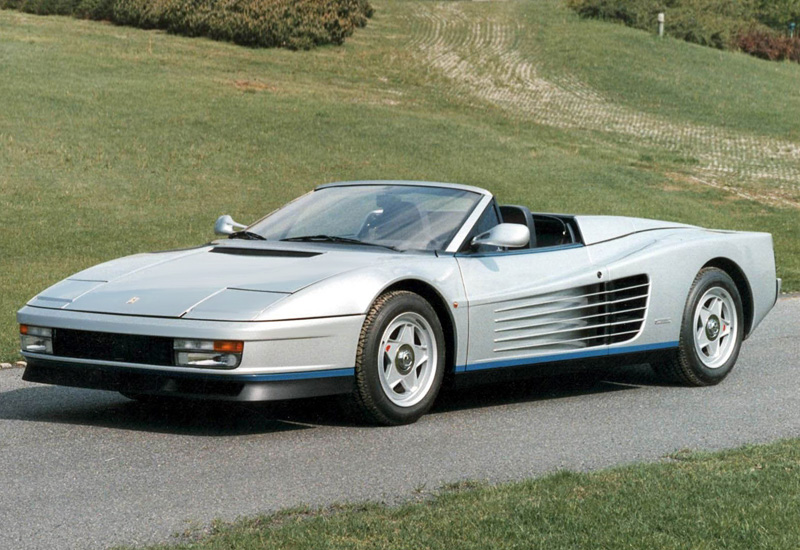
\includegraphics[scale=0.15]{ferrari.jpg}\\
 
 \end{multicols} 
  

}

\subsection{Example - Solution}
\frame{

\frametitle{Example -  Solution}



The {\bf solution} to a differential equation describes the \vspace{2mm}\\ \underline{\hspace{40mm}}\hspace{2mm}\underline{\hspace{40mm}} as a function \vspace{2mm}\\of the \underline{\hspace{40mm}}\hspace{2mm}\underline{\hspace{40mm}}.  \vspace{5mm}\\


	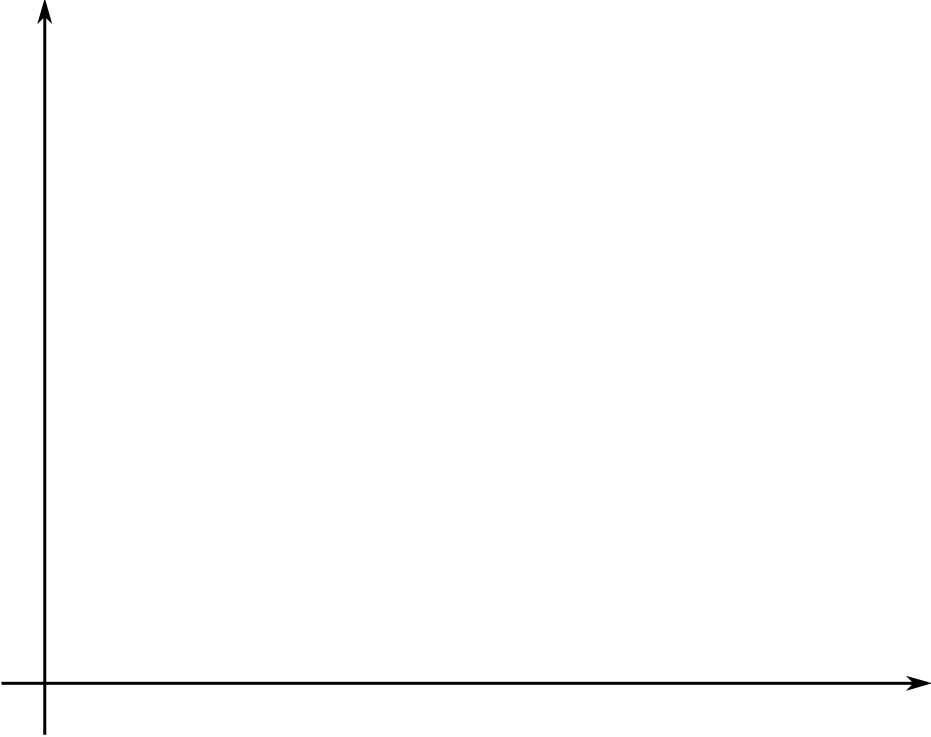
\includegraphics[scale=0.10]{lecture1_fig2.png} \hspace{10mm} 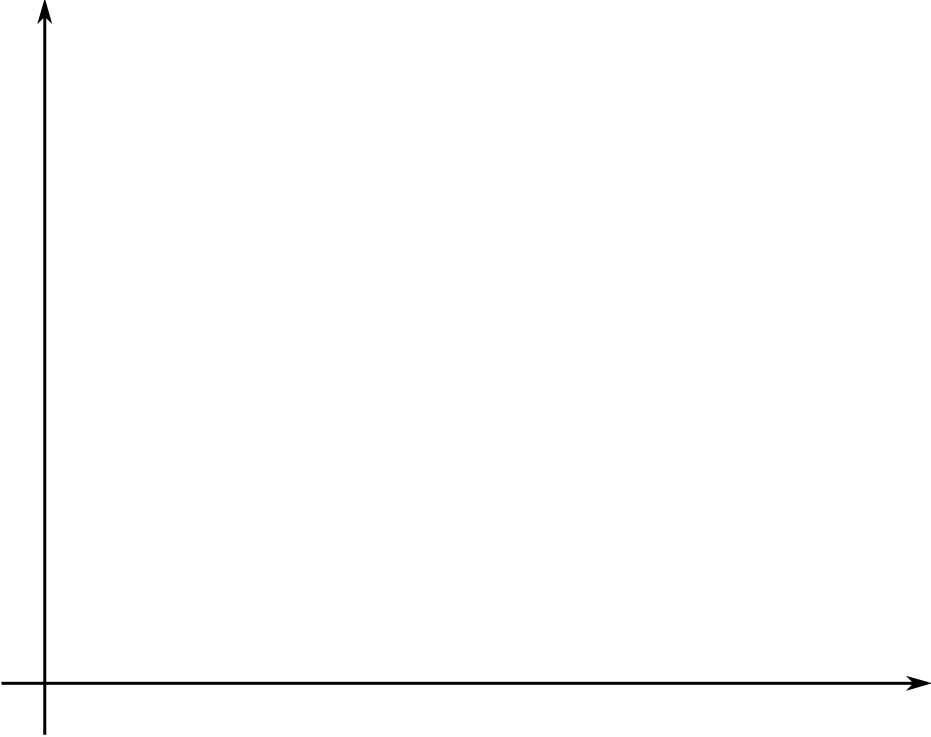
\includegraphics[scale=0.10]{lecture1_fig2.png}\vspace{2mm}\\
	
	%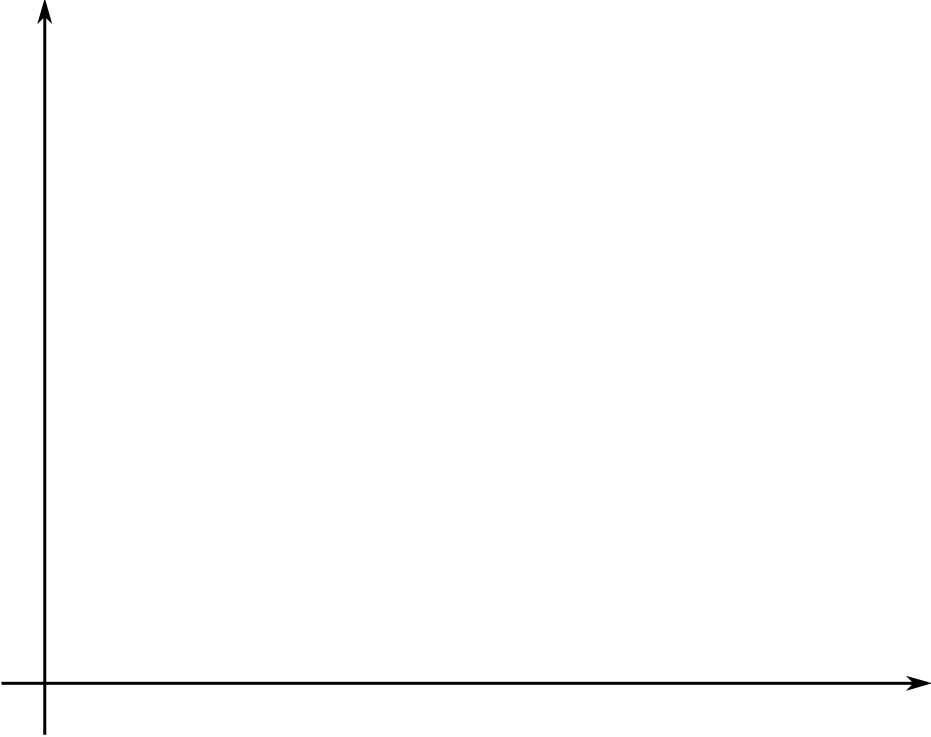
\includegraphics[scale=0.1]{lecture1_fig2.png}\\	
	
There are many different methods for finding the solution.
  

}

\end{document}









